\documentclass{article}
\linespread{1.3}
\usepackage[margin=50pt]{geometry}
\usepackage{amsmath, amsthm, amssymb, amsthm, tikz, fancyhdr, float, graphicx, spverbatim, systeme}
\pagestyle{fancy}
\renewcommand{\headrulewidth}{0pt}
\newcommand{\changefont}{\fontsize{15}{15}\selectfont}

\fancypagestyle{firstpageheader}{
  \fancyhead[R]{
    \changefont
    \parbox[t]{4cm}{ % Adjust width as needed
      Michael Huang\\
      EN.555.644.81\\
      Midterm
    }
  }
}

\begin{document}

\thispagestyle{firstpageheader}
{\Large 

\section*{1.}

\subsection*{(a)} 

The maintenance margin of \$2,000 is only \$1,000 less compared to the initial margin of \$3,000. Therefore, the company cannot lose more than \$1,000 without triggering a margin call. The short futures contract is for 5,000 bushels of wheat, so we therefore know that accordingly for the price at which a margin call will be triggered would be \$1,000 \(\div\) 5,000 = \$0.20, so a price change of 20 cents. In this case, as the company is shorting, a \boxed{\textbf{price increase of 20 cents}} to 470 cents per bushel would trigger a margin call.

\subsection*{(b)}

To withdraw \$1,500, the company would simply need to make \$1,500 on their position, and it cannot go below the initial margin. So in the equivalent position it currently holds, there would need to be a price change of \$1,500 \(\div\) 5,000 = \$0.30, so a price change of 30 cents. Since this is a short, a \boxed{\textbf{price decrease of 30 cents}} to 420 cents per bushel then allow \$1,500 to be withdrawn from the margin account.

}
{\Large 

\section*{2.}

\boxed{\textbf{b., c., d.}} - Convexity increases with the square of maturity, measures the rate of change in duration, and also increases if the coupon on a bond is decreased. \\
Bond convexity decreases as yields decrease, so a. is not true.

}
{\Large 

\section*{3.}

\boxed{\textbf{c.}} - The party with the short positions determines when delivery will take place in a corn futures contract.

}
{\Large 

\section*{4.}

\boxed{\textbf{d.}} - Daily settlement is not a characteristic of a forward contract; this is instead for futures contracts.

}
{\Large 

\section*{5.}

On March 1, the spot price is \$60 and the July futures price is \$59; on June 1, the spot price is \$64 and the July futures price is \$63.50. The company purchases oil on June 1 at a price of \$64, but hedged using a long position to lock in the buying price. The effective price received is 
\[
  S_2 - (F_2 - F_1) = 64 - (63.5 - 59) = 64 - 4.5 = \boxed{\textbf{\$59.50}}
\]

}
{\Large 

\section*{6.}

\boxed{\textbf{b.}} - If a company is hedging the purchase of the underlying asset on June 15, then it should use a futures contract in July. This is because we should be choosing a delivery month that is as close as possible to the hedged transaction, but no earlier than the actual transaction. Delivery isn't guaranteed after June 15 for the June contract, so use July instead.

}
{\Large 

\section*{7.}
To convert from quarterly to semiannual compounding, we solve using \((1 + \frac{R}{m})^m\) for the respective periods:
\[
  (1 + \frac{0.12}{4})^4 = (1 + \frac{R}{2})^2
\]
\[
  (1 + 0.03)^2 = 1 + \frac{R}{2}
\]
\[
  1.0609 = 1 + \frac{R}{2}
\]
\[
  \frac{R}{2} = 0.0609 
\]
\[
  R = 0.1218
\]
So the equivalent rate is \boxed{\textbf{12.18\%}}.

}
{\Large 

\section*{8.}

\boxed{\textbf{b.}} - The short risk-free rate used by traders in the OTC market is usually the LIBOR or SOFR rate. 

}
{\Large 

\section*{9.}

The yield curve is flat at 6\% per annum with semiannual compounding. We aim to find the value of a FRA where the holder receives interest at 8\% per annum for a six-month period on a prinxipal of \$1,000 starting in two years. We know the payoff to be 
\[
  L \cdot (R_K - R_M)(T_2 - T_1)
\]
\[
  = 1000 \cdot (0.08 - 0.06) \cdot (0.5 - 0)
\]
\[
  = 1000 \cdot 0.02 \cdot 0.5 = 10
\]
within those six months. We now discount this back 2.5 years, as the FRA is is for a six-month period the begins in two years. Using semiannual compounding, this gives us
\[
  V = \frac{10}{(1 + \frac{0.06}{2})^(2.5 \cdot 2)}
\]
\[
  V = \frac{10}{(1 + 0.03)^5} = \frac{10}{1.1592740743} = 8.62608784384 \approx \boxed{\textbf{\$8.63}}
\]

}
{\Large 

\section*{10.}

The duration is the maturity of the bond. To calculate the portfolio's duration, we take the weighted average of the portfolio:
\[
  D = \frac{1000 \cdot 5 + 4000 \cdot 10}{1000 + 4000} = \frac{5000 + 40000}{5000} = 9
\]
So the duration of the portfolio is \boxed{\textbf{9 years}}.

}
{\Large 

\section*{11.}

With the spot price of the investment asset providing no income being \$30 and the risk-free rate for all maturities at 10\%, we can calculate the three-year forward price like so: 
\[
  F_0 = S_0e^{rT}
\]
\[
  F_0 = 30 \cdot e^{0.1 \cdot 3} = 30 \cdot e^{0.3} = 30 \cdot 1.34985880758 = 40.4957642274 \approx 40.50
\]
So the price is approximately \boxed{\textbf{\$40.50}}.

}
{\Large 

\section*{12.}

With the additional \$2 income at the end of the first and second year, we adjust accordingly:
\[
  F_0 = (S_0 - I)e^{rT}
\]
First, discounting to get the PV of the income:
\[
  I = 2(e^{-0.10 \cdot 1} + e^{-0.10 \cdot 2}) = 2(e^{-0.10} + e^{-0.20}) = 2(0.90483741803 + 0.81873075307)
\]
\[
  I = 2(1.7235681711) = 3.4471363422
\]
and continuing:
\[
  F_0 = (30 - 3.4471363422)e^{0.10 \cdot 3} = (26.5528636578)e^{0.3} 
\]
\[
  F_0 = 26.5528636578 \cdot 1.34985880758 = 35.842616875 \approx 35.84
\]
So the price is approximately \boxed{\textbf{\$35.84}}.

}
{\Large 

\section*{13.}

If this is instead a forward contract, we use the following:
\[
  f = (F_0 - K)e^{-rT}
\]
Using the previous \(F_0\):
\[
  f = (40.50 - 30)e^{-0.10 \cdot 3} = (10.50)e^{-0.30} 
\]
\[
  f = 10.50 \cdot 0.74081822068 = 7.77859131714 \approx 7.78
\]
So the value of the forward contract is approximately \boxed{\textbf{\$7.78}}.

}
{\Large 

\section*{14.}

If the trader has a long position in one SOFR / Eurodollar futures contract, when the futures price quote increases by 6 basis points, because each contract is standardized to \$1 million notional and \$25 change per basis point, the trader gains \(6 \cdot \$25 = \) \boxed{\textbf{+\$150}}. 

}
{\Large 

\section*{15.}

We have the 9-month rate at 8\% and 6-month rate at 7.5\%. We first get the forward rate for the 6 to 9 month period: 
\[
  R_F = \frac{R_2T_2 - R_1T_1}{T_2 - T_1}
\]
\[
  R_F = \frac{0.08 \cdot \frac{9}{12} - 0.075 \cdot \frac{6}{12}}{\frac{3}{12}}
\]
\[
  R_F = \frac{0.08 \cdot 0.75 - 0.075 \cdot 0.5}{0.25}
\]
\[
  R_F = \frac{0.06 - 0.0375}{0.25} = \frac{0.0225}{0.25} = 0.09
\]
So we have a 9\% rate for the months between 6 and 9 months. The forward interest rate with quarterly compounding becomes 
\[
  4(e^{\frac{0.09}{4}} - 1) = 4(e^{0.0225} - 1) = 4(1.25232271619 - 1) = 0.09102013664 
\]
or 9.102013664\%. The quote would therefore be \(100 - 9.102013664 = 90.897986336 \approx\) \boxed{\textbf{90.90}}.

}
{\Large 

\section*{16.}

\subsection*{a.} 

Looking at the borrowing rates, we see that the spread for each company in the markets differs, despite Company B having better rates overall. So there is some comparative advantage at play: the spread is \(11.0 - 10.6\) = 0.4\% in Sterling and \(7.0 - 6.0\) = 1.0\% in USD. The total benefit to all parties, including the intermediary bank, should be \(1.0 - 0.4\) = 0.6\%, or 60 bp. Breaking this down, we do indeed see that the bank should theoretically be able to take 10 bp, leaving 50 bp = \(2 \cdot 25\) bp, i.e. 25 bp each for the two companies.

\subsection*{b.} 

\begin{figure}[h!]
  \centering
  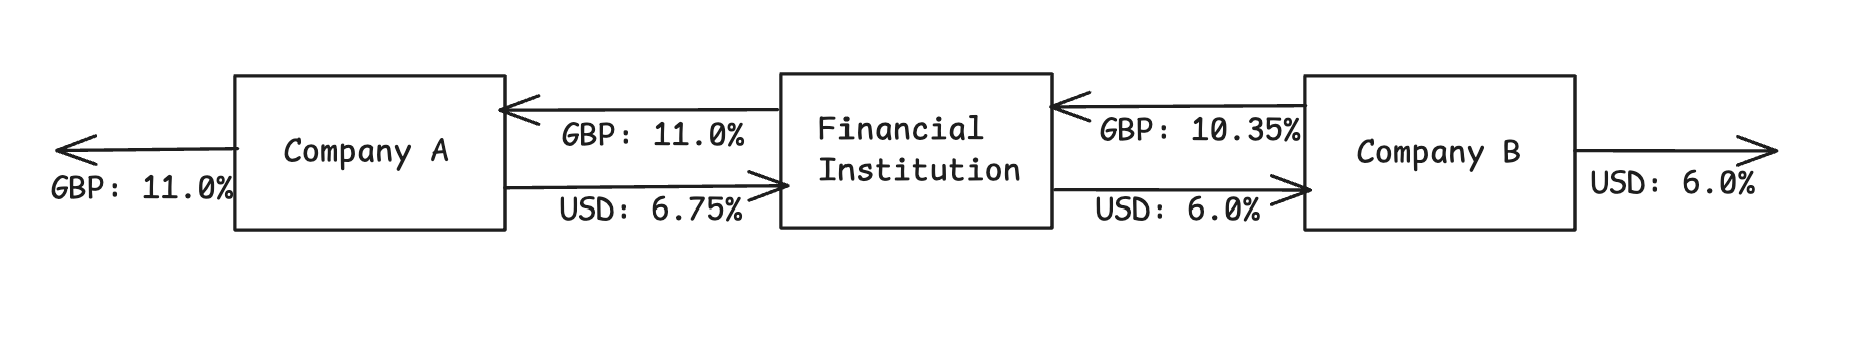
\includegraphics[width=500pt]{16_b_diagram.png}
\end{figure}

\subsection*{c.} 

The bank takes on foreign exchange risk in this case, where the 10 bp gained by the bank can technically shift due to changes in exchange rates between USD and GBP. The bank is losing 65 bp through the GBP leg, but gaining 75 bp through the USD leg. The bank can hedge this risk by using forward contracts to buy an equivalent amount of GBP as they lose on each payment day and therefore lock in the USD gain. 

}
{\Large 

\section*{17.}

The interest rate swap has 9 months left, pays out semi-annually, and compounds semi-annually with fixed rate 5.00\%. The 6-month LIBOR rate observed 3 months ago was 4.85\% with semi-annual compounding. Today's 3- and 9-month LIBOR rates are 5.3\% and 5.8\%, continuously compounded. The forward LIBOR rate for the period between 3 and 9 months is 6.14\% with semi-annual compounding. We aim to find the value of the swap to the party receiving the fixed rate, with an initial principal value of \$15 million. \\ \\
We know that each fixed semiannual coupon pays out \(\frac{0.05}{2} \cdot \) \$15 million = \$375,000. Let's then begin calculating the net at each period: \\
- At 3 months, for the floating leg, we have \(\frac{0.0485}{2} \cdot \) \$15 million = \(0.02425 \cdot 150000000 = \) \$363,750. So the net is \$375,000 - \$363,750 = \$11,250. \\
- At 9 months, for the floating leg, we have \(\frac{0.0614}{2} \cdot \) \$15 million = \(0.0307 \cdot 15000000 = \) \$460,500. So the net is \$375,000 - \$460,500 = -\$85,500. \\
Discounting these net flows using the continuously-compounded rates, we have 
\[
  V = 11250 \cdot e^{-0.053 \cdot \frac{3}{12}} - 85500 \cdot e^{-0.058 \cdot \frac{9}{12}}
\]
\[
  V = 11250 \cdot e^{-0.053 \cdot 0.25} - 85500 \cdot e^{-0.058 \cdot 0.75}
\]
\[
  V = 11250 \cdot e^{-0.01325} - 85500 \cdot e^{-0.0435}
\]
\[
  V = 11250 \cdot 0.98683739483 - 85500 \cdot 0.95743255409
\]
\[
  V = 11101.9206918 - 81860.4833747 = -70758.5626829 \approx -70758.56
\]
So the fixed rate receiver values the swap at approximately \boxed{\textbf{-\$70,758.56}}, i.e. they lose approximately that much. 

}
\end{document}